\chapter{ΕΡΩΤΗΜΑ 1}

    \section{ΕΡΓΑΛΕΙΑ ΓΙΑ ΧΕΙΡΙΣΜΟ ΠΡΟΒΛΗΜΑΤΩΝ ΒΙΟΠΛΗΡΟΦΟΡΙΚΗΣ}

        Η σελίδα της Rosalind περιλαμβάνει κάποια βασικά προβλήματα με σκοπό μια πρώτη εξοικείωση στο τομέα της Βιοπληροφορικής.

    \subsection{"Introduction to the Bioinformatics Armory": (SMS 2)}
        Το πρώτο πρόβλημα αφορά την εύρεση των αριθμών των νουκλεοτιδίων από μια ακολουθία DNA.
        Ένα εργαλείο για την ανάλυση της ακολουθίας είναι το Sequence Manipulation Suite (SMS) 2.
        Πρόκειται για μια συλλογή Javascript προγραμμάτων για τη δημιουργία, στοίχιση και ανάλυση μικρών DNA και πρωτεϊνικών ακολουθιών. \cite{SMS2}
        Χρησιμοποιώντας το DNA Stats, εισάγουμε το Sample Dataset και εισάγεται το πλήθος των νουκλεοτιδίων, και το ποσοστό εμφάνισής τους:
        \vspace{-10pt}
        \begin{table}[ht] \noindent\centering\tt
        \resizebox{0.4\textwidth}{!}{
            \begin{tabular}{lll}
            Pattern & Times found: & Percentage \\
            \midrule
            g & 17 & 24.29 \\
            a & 20 & 28.57 \\
            c & 21 & 30 \\
            3 & 12 & 17.14 \\
            \end{tabular}}
        \end{table}
        \vspace{-10pt}

    \subsection{"GenBank Introduction": Αναζήτηση}
        Αφορά τη βάση δεδομένων GenBank. \cite{GenBank} Μπορούμε να αναζητήσουμε ακολουθίες νουκλεοτιδίων και πρωτεϊνών, όπως επίσης και βιβλιογραφικές δημοσιεύσεις.

    \subsection{"Data Formats": Formats της GenBank}
        Στην GenBank για να υπάρχει μια συνέπεια στην αναπαράσταση των νουκλεοτιδικών ακολουθιών ακολουθείται ένα συγκεκριμένο format με ορισμένο header, τα χαρακτηριστικά της ακολουθίας και την ίδια την ακολουθία.
        Μέσω του εργαλείου GenBank to Fasta του SMS 2 \cite{GenBankToFASTA} μπορούμε να αντιγράψουμε κάποιο entry από το GenBank και να το μετατρέψουμε σε FASTA, την κλασική αναπαράσταση νουκλεοτιδίων.
        Για παράδειγμα:

\begin{graycomment} \footnotesize
    \begin{verbatim}
GenBank to FASTA results
>Strongylocentrotus purpuratus fascin (FSCN1) mRNA, complete cds.
acttgaaagtggataaaatcgactgataccaaaacaacattgttttacagaagtggtcgt
ttgaggacatcaacatatttcacaatgcctgctatgaatttaaaatacaaatttggcctg\end{verbatim}
\end{graycomment}

    \subsection{"New Motif Discovery": Αναζήτηση Motifs σε ακολουθίες}
        Με το εργαλείο MEME (Multiple Em for Motif Elicitation) \cite{MEME}, εισάγοντας ακολουθίες που περιλαμβάνει motif (δηλαδή ένα επαναλαμβανόμενο μοτίβο), εξάγεται η κανονική έκφραση του συγκεκριμένου motif.

    \subsection{"Pairwise Global Alignment": Στοίχιση ακολουθιών}
        Στο εργαλείο Needle \cite{Needle} μπορούμε να εισάγουμε τα ID από δύο GenBank entries. Κομμάτι του αποτελέσματος που εξάγεται:
\begin{graycomment} \footnotesize
            \begin{verbatim}
%# Length: 142
%# Identity:     122/142 (85.9%)
%# Similarity:   131/142 (92.3%)
%# Gaps:           0/142 ( 0.0%)
%# Score: 648.0 \end{verbatim}
\end{graycomment}


    \subsection{"FASTQ format introduction": Μετατροπή FASTQ σε FASTA}
        Ένα FASTQ αρχείο είναι μια μορφή αρχείου που αποθηκεύει μια ακολουθία και επιπλέον πληροφορία για αυτή (quality scores).
        Υπάρχουν διαφορετικοί online convertors που μπορούν να το μετατρέψουν σε FASTA, όπως ο Sequence Conversion της Bugaco, \cite{BugacoConversion} στον οποίον ανεβάζουμε ένα FASTQ αρχείο και το μετατρέπουμε σε αρχείο \texttt{.fasta}.

    \subsection{"Read Quality Distribution": Per sequence quality analysis}
        Το FastQC \cite{FastQC} είναι λογισμικό ανάγνωσης ακολουθιακών δεδομένων, το οποίο μπορεί να εξάγει γραφικά και πίνακες ελέγχου ποιότητας των ακολουθιών.
    \begin{graycomment} \footnotesize
    \begin{verbatim}
INPUT:
    @Rosalind_0041
    GGCCGGTCTATTTACGTTCTCACCCGACGTGACGTACGGTCC
    +
    6.3536354;.151<211/0?::6/-2051)-*"40/.,+%)
    @Rosalind_0041
    TCGTATGCGTAGCACTTGGTACAGGAAGTGAACATCCAGGAT
    +
    AH@FGGGJ<GB<<9:GD=D@GG9=?A@DC=;:?>839/4856
    @Rosalind_0041
    ATTCGGTAATTGGCGTGAATCTGTTCTGACTGATAGAGACAA
    +
    @DJEJEA?JHJ@8?F?IA3=;8@C95=;=?;>D/:;74792\end{verbatim}
    \end{graycomment}
    \begin{center} \noindent
        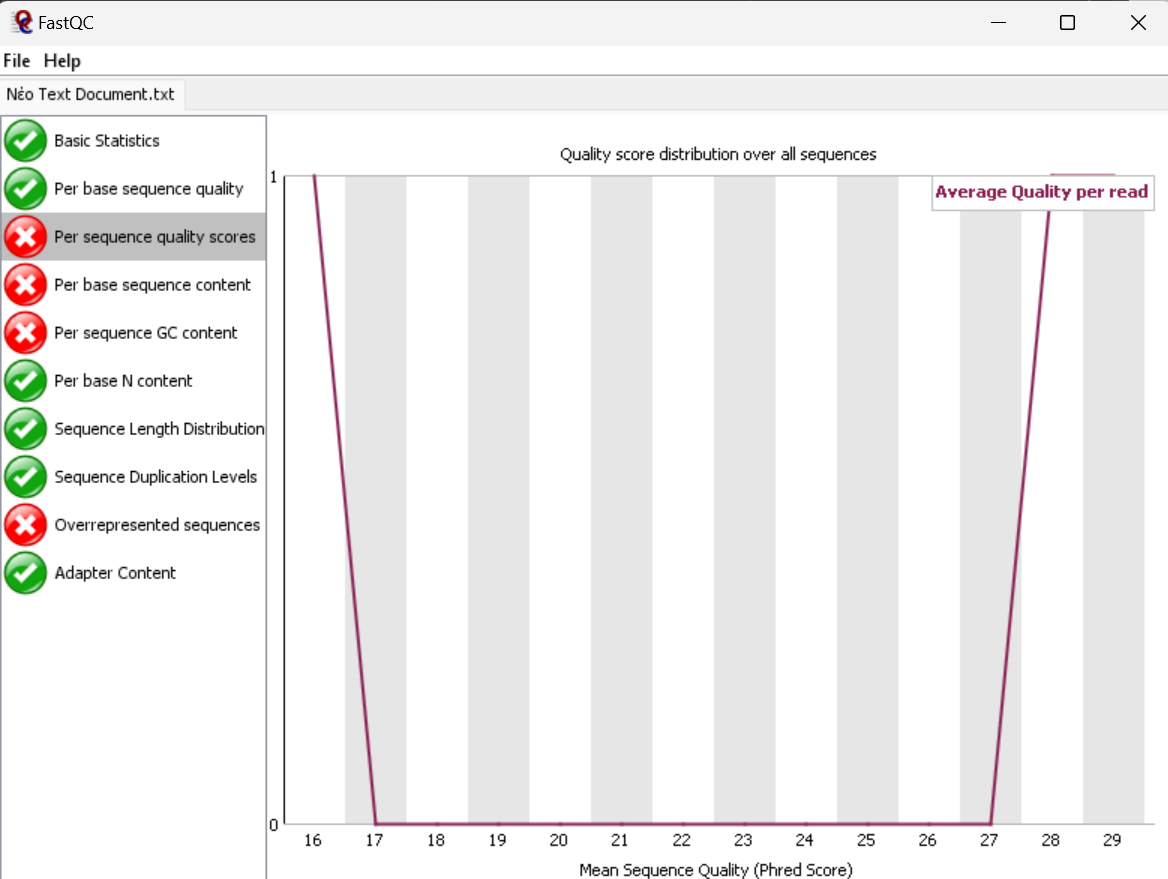
\includegraphics[scale=0.4]{img/FastQC}
    \end{center}

    \subsection{"Protein Translation": SMS 2 Translate}
        Μέσω του εργαλείου Translate του SMS 2 \cite{Translate}, μπορούμε να μεταφράσουμε την αλληλουχία των νουκλεοτιδίων σε αμινοξέα. Για παράδειγμα:

\begin{graycomment} \footnotesize
    \begin{verbatim}
INPUT:
    >test
    ATGGCCATGGCGCCCAGAACTGAGATCAATAGTACCCGTATTAACGGGTGA
OUTPUT:
    >rf 1 test
    MAMAPRTEINSTRING*
\end{verbatim}
\end{graycomment}

    \subsection{"Read Filtration by Quality": FASTQ Quality Filter}
        Μπορούμε να "καθαρίσουμε" entries χρησιμοποιώντας συγκεκριμένο threshold (quality cut-off value και ποσοστό entries που να ικανοποιούνται από αυτό) χρησιμοποιώντας το FASTQ Quality Filter της Galaxy. \cite{GalaxyFastQQualityFliter}
        Εξάγεται το αρχείο \verb|Galaxy2-[Filter_by_quality_on_data_1].fastqsanger| το οποίο περιλαμβάνει μόνο τα φιλταρισμένα entries.

    \subsection{"Complementing a Strand of DNA": SMS 2 Reverse Complement }
        Το Reverse Complement του SMS 2 επιστρέφει τα συμπληρωματικά νουκλεοτίδια. Για παράδειγμα:
\begin{graycomment} \footnotesize
    \begin{verbatim}
INPUT:
    >Rosalind_12
    GACTCCTTTGTTTGCCTTAAATAGATACATATTTACTCTTGACTCTTTT...
    ...GTTGGCCTTAAATAGATACATATTTGTGCGACTCCACGAGTGATTCGTA
    >Rosalind_37
    ATGGACTCCTTTGTTTGCCTTAAATAGATACATATTCAACAAGTGTGCA...
    ...CTTAGCCTTGCCGACTCCTTTGTTTGCCTTAAATAGATACATATTTG
OUTPUT:
    The best non-identical alignments are:     ls-w bits E(1) %_id  %_sim  alen
    Rosalind_37                     (  96) [f]  465 35.8 1.6e-07 0.763 0.774   93
    +-                                          308 19.1   0.017 0.549 0.593   91
    +-                                          252 13.1    0.65 0.476 0.563  103
    +-                                          244 12.3    0.85 0.489 0.564   94
    +-                                          235 11.3    0.98 1.000 1.000   34
    Rosalind_37                     (  96) [r]  229 10.7       1 0.442 0.526   95\end{verbatim}
\end{graycomment}

    \subsection{"Suboptimal Local Alignment": Lalign}
        Το εργαλείο Lalign \cite{Lalign} βρίσκει επαναλαμβανόμενες εσωτερικές ακολουθίες νουκλεοτιδίων ή πρωτεϊνών, στοιχίζοντας ξένες υπακολουθίες ψάχνοντας ομοιότητες. Για παράδειγμα:
\begin{graycomment} \footnotesize
    \begin{verbatim}
INPUT:
    >Rosalind_48
    GCATA
OUTPUT:
    >Rosalind_48 reverse complement
    TATGC\end{verbatim}
\end{graycomment}


    \subsection{"Base Quality Distribution": Per Base Sequence Quality}
        Το FastQC \cite{FastQC} εμφανίζει διάγραμμα με τη μετρική Base Call Quality. Για παράδειγμα:
    \begin{graycomment} \footnotesize
         \begin{multicols}{2} \centering
             \begin{verbatim}
INPUT:
    @Rosalind_0029
    GCCCCAGGGAACCCTCCGACCGAGGATCGT
    +
    >?F?@6<C<HF?<85486B;85:8488/2/
    @Rosalind_0029
    TGTGATGGCTCTCTGAATGGTTCAGGCAGT
    +
    @J@H@>B9:B;<D==:<;:,<::?463-,,
    @Rosalind_0029
    CACTCTTACTCCCTAGCCGAACTCCTTTTT
    +
    =88;99637@5,4664-65)/?4-2+)$)$
    @Rosalind_0029
    GATTATGATATCAGTTGGCTCCGAGAGCGT
    +
    <@BGE@8C9=B9:B<>>>7?B>7:02+33.
             \end{verbatim}
        \end{multicols}
    \end{graycomment}

    \begin{center} \noindent
        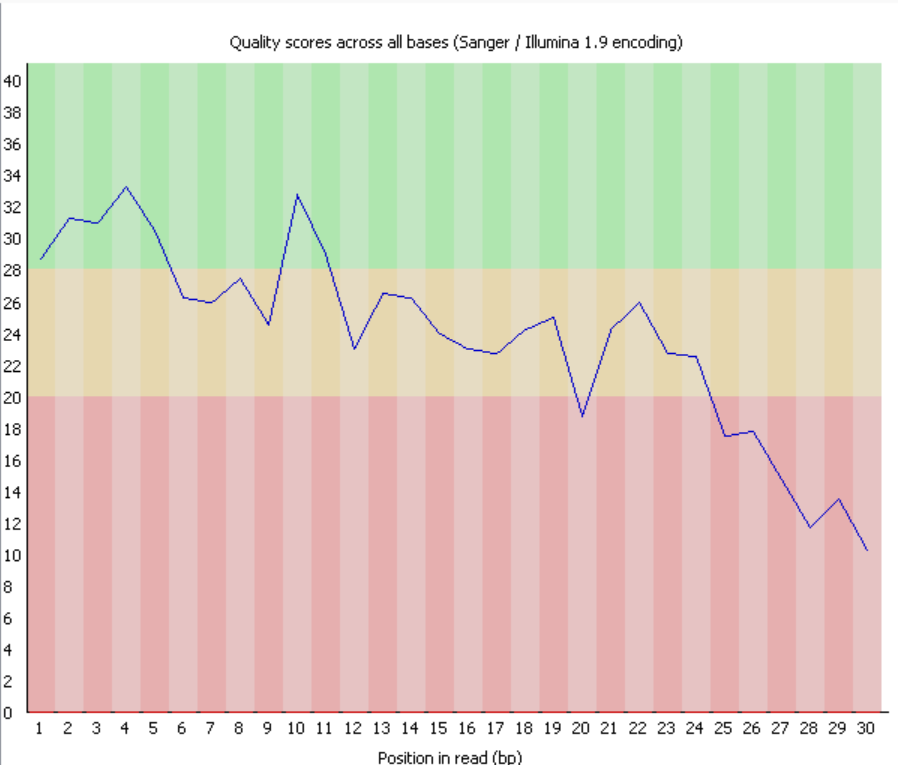
\includegraphics[scale=0.5]{img/Per Base Sequence Quality}
    \end{center}

    \subsection{"Global Multiple Alignment": Clustal}
        Το πρόγραμμα Clustal πραγματοποιεί στοίχιση ακολουθιών.
    \begin{graycomment} \footnotesize
    \begin{verbatim}
OUTPUT:
    Rosalind_7       -----CACGTCTGTTCGCCTAAAACTTTGATTGCCGGCCTACGCTAGTTAGTTA	49
    Rosalind_28      GGGGTCATGGCTGTTTGCCTTAAACCCTTGGCGGCCTAGCCGTAATGTTT----	50
    Rosalind_51      --TCCTATGTTTGTTTGCCTCAAACTCTTGGCGGCCTAGCCGTAAGGTAAG---	49
    Rosalind_18      ---GACATGTTTGTTTGCCTTAAACTCGTGGCGGCCTAGCCGTAAGTTAAG---	48
    Rosalind_23      --ACTCATGTTTGTTTGCCTTAAACTCTTGGCGGCTTAGCCGTAACTTAAG---	49
                           * *  **** **** ****       * *            *\end{verbatim}
    \end{graycomment}

    \subsection{"Finding Genes with ORFs": }
        Το OTF Finder του SMS 2 ξεχωρίζει το κωδικόνιο έναρξης και λήξης και επιστρέφει τη μεγαλύτερη πρωτεϊνική ακολουθία. Για παράδειγμα:
\begin{graycomment} \footnotesize
    \begin{verbatim}
INPUT:
    >sample sequence
    gcggcggcggcggcggcggcggcggcggcggcggcggcggcggcggcggcggcggcggcggcggcggcggcggcggcg...
OUTPUT:
>Translation of ORF number 1 in reading frame 1 on the direct strand.
AAAAAAAAAAAAAAAAAAAAAAAAAAAAAA*\end{verbatim}
\end{graycomment}

    \subsection{"Base Filtration by Quality": }
        Το FASTQ Quality Filter του Galaxy μπορεί να χρησιμοποιηθεί για να καθαρίσουμε τα entries που δεν ικανοποιούν κάποιο threshold.
        Για παράδειγμα για window size 20:
    \begin{graycomment} \footnotesize
    \begin{verbatim}
INPUT:
    @Rosalind_0049
    GCAGAGACCAGTAGATGTGTTTGCGGACGGTCGGGCTCCATGTGACACAG
    +
    FD@@;C<AI?4BA:=>C<G=:AE=><A??>764A8B797@A:58:527+,
OUTPUT:
    @Rosalind_0049
    GCAGAGACCAGTAGATGTGTTTGCGGACGGTCGGGCTCCATGTGACAC
    +
    FD@@;C<AI?4BA:=>C<G=:AE=><A??>764A8B797@A:58:527\end{verbatim}
    \end{graycomment}


    \section{ΒΑΣΕΙΣ ΔΕΔΟΜΕΝΩΝ NCBI \& EBI}
        Η βάση δεδομένων NCBI (National Center for Biotechnology Information) \cite{NCBI} χρησιμοποιεί το COBALT \cite{COBALT} ως εργαλείο πολλαπλής στοίχισης.
        ΤΟ COBALT (Constraint-Based Multiple Alignment Tool) χρησιμοποιεί motif μοτίβα και ομοιότητες από υπάρχουσες βάσεις δεδομένων, τα οποία μετά αξιοποιεί για τη στοίχιση των ακολουθιών.
        Είναι πιο αποτελεσματικό σε συγκεριμένα είδη πρωτεϊνών.

        Αντίθετα, η βάση δεδομένων EBI \cite{EBI} (European Bioinformatics Institute) χρησιμοποιεί το Cluster Omega \cite{ClusterOmega}.
        Το Cluster Omega είναι εξαιρετικά γρήγορο και ευέλικτο καθώς χρησιμοποιεί ιεραρχικές δομές (guide trees) που αναπαριστούν τις συσχετίσεις μέσα στην ακολουθία.
        Μπορεί να στοιχίσει ταυτόχρονα πολλαπλές ακολουθίες, έχοντας ως αποτέλεσμα τον εντοπισμό διατηρημένων περιοχών σε διαφορετικές αλληλουχίες, προσφέροντας υψηλή ακρίβεια και κλιμακωτή απόδοση.